%% Technical Report for the work on the AI-DSL over the period of May
%% to September 2022.

\documentclass[]{report}
\usepackage{amssymb}
\usepackage{url}
\usepackage{minted}
\usepackage[textsize=footnotesize]{todonotes}
\newcommand{\kabir}[2][]{\todo[color=yellow,author=kabir, #1]{#2}}
\newcommand{\nil}[2][]{\todo[color=purple,author=nil, #1]{#2}}
\usepackage[hyperindex,breaklinks]{hyperref}
\usepackage{breakurl}
\usepackage{listings}
\lstset{basicstyle=\ttfamily\footnotesize,breaklines=false,frame=single}
\usepackage{float}
\restylefloat{table}
\usepackage{longtable}
\usepackage{graphicx}
\usepackage[font=small,labelfont=bf]{caption}
\usepackage[skip=0pt]{subcaption}
\usepackage{circledsteps}

\begin{document}

\title{AI-DSL Technical Report\\(May to Septembre 2022) \[\texttt{DRAFT}\]}
\author{Nil Geisweiller, Samuel Roberti, Matthew Ikl\'e, Deborah Duong}
\maketitle

\begin{abstract}
\end{abstract}

\tableofcontents

\chapter{Introduction}

\section{Setting the Scene}

In the previous iteration we explored using Dependent Types to express
formal specifications of AI services, with the ultimate goal of
building a language for easily writing those specifications, the
AI-DSL itself, as well as services to automatically connect AI
services together, the AI-DSL Registry~\cite{AIDSLReport2021}.

Back then we experimented with trivial AI services, computing simple
arithmetic, described by trivial properties, such as the parity of
their inputs/outputs.  We were able to demonstrate that Idris, our DTL
of choice, could be used to verify the correctness of such AI service
assemblages.  The approach seemed promising, but to really put the
idea to the test we had to make progress on two fronts:

\begin{enumerate}
\item Replace trivial AI services by actual AI algorithms.
\item Explore program synthesis, as it became clear that it was at the
  heart of this endeavor.  First, for building the AI service
  assemblages themselves.  Second, for achieving fuzzy matching, that
  is when AI services almost fit together but not quite yet.  And
  third, for completing assemblages when some AI services are outright
  missing.
\end{enumerate}
That is what we have done during that iteration.

\section{Work Accomplished}

First we have implemented three AI algorithms in Idris:
\begin{enumerate}
\item Gradient descent
\item Linear regression
\item Logistic regression
\end{enumerate}
These algorithms were chosen because they are relatively simple, yet
extensively use in real world applications, as well as tightly related
to each other.  Linear regression can be framed as a gradient descent
problem, and logistic regression can be framed both as gradient
descent and linear regression problems, thus constituting an excellent
case study for the AI-DSL.  Alongside these implementations, a
descending property was formulated and formally proved for each
algorithm.

Finally, we have explored ways to perform program synthesis of
dependently typed programs.  While we have only achieved partial
success as far as program synthesis is concerned, we were able to
demonstrate its feasibility within the Idris ecosystem.  It was clear
from the start anyway that to be done well and fully, program
synthesis essentially requires achieving AGI.  Indeed, it is one of
these AI-complete problems.  That is any problem can be framed as a
program synthesis problem and vice versa.  The idea being that such
functionality can be progressively grown, deferred less and less to
human intervention, as the network and the AI-DSL evolve.

\section{Related Work}

Here's a list of projects and publications we have discovered along
the way that relate to the work done during that iteration.

\subsection{Machine Learning Formal Verification}

The most relevant work we have found so far is described in a paper
entitled \emph{Developing Bug-Free Machine Learning Systems With
  Formal Mathematics}~\cite{DBLP:journals/corr/SelsamLD17}.  In that
paper a formal specification of a class of stochastic gradient descent
algorithms operating on stochastic computation graphs is implemented
in Lean~\cite{Lean}, alongside a property expressing that the back
propagation correction points, in average, towards the gradient
descent of the cost.  Mathematically, this may be expressed by the
following equality
$$\mathbb{E}_{g,\theta}[\texttt{bprop}(g,\theta,\bold{X})] = \nabla_{\theta}(\mathbb{E}_{g,\theta}[\texttt{cost}(g,\bold{X})])$$
where $g$ is a stochastic computation graph parameterized by $\theta$,
$\bold{X}$ is a random vector describing the values sampled from $g$,
$\texttt{bprop}$ the is back propagation function and $\texttt{cost}$
is the cost function.  Such equality is formally expressed in Lean
using existing and introduced mathematical vocabulary to express
notions of probability and measure theory such as expectation,
integration and derivation, then proved using tactics developed for
that purpose.  The authors admit that their prove assumes
infinite-precision real numbers as opposed to finite-precision
floating point numbers used in practice.  However, they point to a
couple of papers addressing the use of floating point numbers in the
context of automatic theorem proving~\cite{Harrison2006,
  Ramananandro2016}.

Another related work presented in~\cite{Bagnall2019} aims to prove
properties about learned models, as opposed to learning algorithms.
Formalizing Hoeffding's inequality~\cite{Hoeffding1963} in
Coq~\cite{Bertot2004}, the authors show how to automatically prove the
extend to which a given model, such as a perception, generalizes on
unknown data.

TODO: mention various relevant Idris projects.

% - [ ] Mention the following Idris2 packages
%   - [ ] https://github.com/stefan-hoeck/idris2-graph
%   - [ ] https://github.com/idris-bayes/log-domain
%   - [ ] https://github.com/idris-bayes/prob-fx
%   - [ ] https://github.com/madman-bob/idris2-jupyter
%   - [ ] https://github.com/joelberkeley/spidr
%   - [ ] https://github.com/stefan-hoeck/idris2-prim
%   - [ ] https://github.com/madman-bob/idris2-python
% - [ ] Newton, Preconditioning, step size cycling scheduling, etc
% - [ ] ConCert https://arxiv.org/pdf/1907.10674.pdf
% - [ ] A Coq-based synthesis of Scala programs which are
%   correct-by-construction
%   https://cedric.cnam.fr/fichiers/art_4027.pdf
%   https://github.com/JBakouny/Scallina
% - [ ] https://stackoverflow.com/questions/23436823/converting-coq-to-idris
% - [ ] See paper Learning to Prove Theorems via Interacting with
%   Proof Assistants
% - [ ] http://ace.cs.ohio.edu/~gstewart/mlcert.html
% - [ ] The AI-DSL is a language of composition, not application!!!
% - [ ] Look into AGDA https://wiki.portal.chalmers.se/agda/pmwiki.php
% - [ ] https://epistasislab.github.io/tpot/

\subsection{Smart Contract Formal Verification}

Over the past years the subject of formal verification of smart
contract has also gathered some attention.

A formal specification of the Ethereum Virtual Machine (EVM) has been
provided~\cite{Hildenbrandt2018} using the $\mathbb{K}$
framework~\cite{Xiaohong2019}, enabling formal verification based on
Reachability Logic~\cite{Alechina2000}.

Approaches for doing formal verification on higher level languages
targeting the EVM also exist.  In 2016 a Master's
thesis~\cite{Pettersson2016} was conducted to explore how Idris can be
used to write smart contracts avoiding common failures such as stack
overflow or lack of cryptographic encryption when required.  On top of
using Idris to detect such failures, the authors extended the Idris
compiler to support Serpent~\cite{Delmolino2015}, a high level
language for the EVM.  To our knowledge unfortunately that work has
not been pursued any further.  Similarly, a system called,
ConCert~\cite{Annenkov2020} has been developed to do formal
verification of smart contracts written in $\lambda_{smart}$, a
fragment of the \textsc{Acorn} smart contract language, using
Coq~\cite{Bertot2004}.

Then they are blockchains that have been created to support formal
verification more or less from the beginning.  Tezos~\cite{Tezos2014},
using Michelson, a stack-based low level smart contract language, now
comes with a formal verification tool called
Mi-Cho-Coq~\cite{Bernardo2019} developed in Coq.  Higher level
languages targeting Michelson also exist such as
Albert~\cite{Bernardo2020}, an Intermediate Level Language, and
Juvix~\cite{Goes2020} a Dependently Typed Language (DTL) based on
Quantitative Type Theory (QTT)~\cite{Atkey2018} that not only allows
to reason about smart contracts at a high level, but also produces
optimized Michelson code by taking advantage of the quantitative
aspect of QTT.  \textsc{Zilliqa}~\cite{Zilliqa2017} comes with
\textsc{Scilla}~\cite{Ilya2018}, an intermediate-level language
enabling formal verification with Coq.  The Zen
protocol~\cite{Zen2017} also supports formal verification via
F*~\cite{Swamy2013}.  Notably, the type of verification described in
its white paper also includes computational resources, to formally
guaranty that a contract will be allocated enough gaz before it is
run.

These are the main publications we have found so far, although a few
more can be found in that study~\cite{Pace2020}, as well as other
articles from that same book of proceedings.  It is a rapidly growing
field and there is no doubt that formal verification will
progressively become an indissociable part of the blockchain
technology.

\subsection{Program and Proof Synthesis}

As far as we can tell, the literature on that subject, that is
automatically synthesizing programs and proofs satisfying a formal
description, is very lacking.  The reasons probably being that it is a
hard problem and language frameworks, such as Idris, dedicated to that
are fairly new.  It seems the best publication on the matter is the
Idris hand book~\cite{Brady2017}.

There is other related work such as Magic Haskell~\cite{} although
fairly limited since such system only supports case-based descriptions
due to the lack of expressive power of Haskell.  There is other
similar work coming from the Inductive Programming Logic community,
essentially suffering from the same limitations as Magic Haskell.

MOSES
https://cseweb.ucsd.edu/~npolikarpova/

Component-based synthesis, or modular synthesis.

Probably the most relevant work we have found regarding program
synthesis can be found in~\cite{Guo2022}.  In this work, RESTful APIs
function calls are composed to fulfill a given specification.  Since
RESTful types are rather limited, their system begins by enhancing
type signatures with \emph{Semantic Types}, exploiting the RESTful
type descriptions to heuristically replace non-semantic types like
\texttt{String} by semantic types like \texttt{User} or \texttt{Id}.
Then performs
% TODO: shouldn't Type Transition Nets be Abstract Transition Networks?
component-based synthesis using Type Transition Nets
(TTN)~\cite{Feng2017, Guo2020}, a special kind of Petri Nets.  Since
Semantic Types are still rather limited, at least compared to
Dependent Types, their system also uses input-output examples to
further narrow down the search.  Overall, it is a very relevant work
and contains parts that could potentially be reused, such as the
TTN-based search.

The last one is not program synthesis per say but rather program
specification synthesis using Liquid Types, short for \emph{Logically
  Qualified Data Types}~\cite{Rondon2008}.  Liquid Types are a
decidable fragment of Refinement Types.  Their system was able to
automatically infer the correct specifications of all functions of an
Array OCAML library.  A bug that had remained hidden so far was
revealed and corrected in the process.  This work could potentially be
used to infer the specifications of existing AI services that can then
be manually corrected, which is easier than having to write a
specification from scratch.

\subsection{Comparing Formal Languages}

The reader may have noticed in these publications the use of other
language frameworks beside Idris, such as Lean, Coq and F*.  It is
still not completely clear what are the pros and cons of each
framework and is something we intend to investigate further.  However
already some observations can be made.  Lean and Coq are more oriented
towards proving mathematical theorems, while Idris is more oriented
towards writing and verifying programs.

The advantage of Idris, as far as we have experienced, is that proofs
and programs are based on the same language, and in fact share a lot
vocabulary.  For instance the function \texttt{map}, from the
\texttt{Functor} interface, may be used inside proofs or programs
alike.  Beside being very elegant, it brings the notion of reusability
to a new level.  It should be noted that Juvix~\cite{Goes2020},
although dedicated to smart contract programming, is very closed
conceptually to Idris.  It is a fairly new language and we may want to
keep a close eye on its development.

Lean and Coq have other advantages, such as having large libraries of
mathematical theories that can be reused when proving properties of
programs.  There is no doubt that Idris mathematical library will grow
but as of today it is lagging behind.

\chapter{Implementation and Verification of AI Algorithms}

\section{Implementation of AI Algorithms}
We have implemented the following AI algorithms in Idris:
\begin{enumerate}
\item Descent: a generic descending algorithm.
\item Gradient Descent: a gradient descent algorithm using Descent.
\item Linear Regression: a linear regression algorithm using Gradient
  Descent.
\item Logistic Regression: a logistic regression algorithm using
  Gradient Descent.
\item Logistic-Linear Regression: a logistic regression algorithm
  using Linear Regression.
\end{enumerate}
\begin{figure}[H]
  \centering
  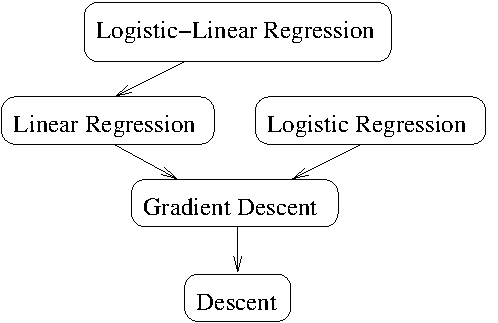
\includegraphics[scale=0.8]{figs/ai-algorithms.xfig.pdf}
  \caption{AI algorithms call graph}
  \label{fig:ai_algorithms}
\end{figure}
A call graph is provided in Figure~\ref{fig:ai_algorithms}.  Each
algorithm may be viewed as an AI service, together forming a network
of AI services delegating work to one another when possible.

The idea of performing logistic regression via two paths, either
directly via calling Gradient Descent, or indirectly via calling
Linear Regression, came from the ambitious goal of having our AI-DSL
prototype discover an alternate way, possibly unforeseen by the AI
practitioner, to perform a certain AI tasks, here logistic regression.
As we will see we did not come far enough to achieve that goal, but we
certainly keep on the side for the future.

Let us now describe in more details what these algorithms are doing,
and then provide the descending property we have focused on in this
work.

\subsection{Descent}
The Descent algorithm takes in input:
\begin{enumerate}
\item a cost function to minimize;
\item a step function to jump from candidate to candidate;
\item an initial candidate to start the search from;
\item a maximum number of steps allocated to the search;
\end{enumerate}
and outputs the final candidate as well as the remaining unallocated
steps.

\subsection{Gradient Descent}
The Gradient Descent algorithm takes in input:
\begin{enumerate}
\item a loss function;
\item a gradient function;
\item a learning rate, also called step size;
\item an initial candidate to start the search from;
\item a maximum number of steps allocated to the search;
\end{enumerate}
converts the gradient function and the learning rate into a step
function, calls the Descent algorithm and returns the final candidate
as well as the remaining unallocated steps.

\subsection{Linear Regression}
The Linear Regression algorithm takes in input:
\begin{enumerate}
\item a data set to explain, a matrix of inputs and a column vector
  of outputs;
\item a learning rate, also called step size;
\item an initial candidate to start the search from;
\item a maximum number of steps allocated to the search;
\end{enumerate}
defines a sum-of-squared-errors-based loss and gradient functions for
that data set, calls Gradient Descent and returns the final candidate
as well as the remaining unallocated steps.

\subsection{Logistic Regression}
The Logistic Regression algorithm takes in input:
\begin{enumerate}
\item a data set to explain, a matrix of inputs and a Boolean column
  vector of outputs;
\item a learning rate, also called step size;
\item an initial candidate to start the search from;
\item a maximum number of steps allocated to the search;
\end{enumerate}
defines a cross-entropy-based loss and gradient functions for that
data set, calls Gradient Descent and returns the final candidate as
well as the remaining unallocated steps.

\subsection{Logistic-Linear Regression}
The Logistic-Linear Regression algorithm takes in input:
\begin{enumerate}
\item a data set to explain, a Boolean matrix of inputs and a Boolean
  column vector of outputs;
\item a learning rate, also called step size;
\item an initial candidate to start the search from;
\item a maximum number of steps allocated to the search;
\end{enumerate}
transforms the data set so that the column vector of outputs
represents the odds of outputting True instead of a Boolean value,
calls linear regression on that transformed data set and returns the
final candidate as well as the remaining unallocated steps.

\section{Verification of AI Algorithms}

The concept of verifying properties of AI algorithms is a very broad
one, could be verifying the AI algorithms themselves, or their output
models, either using crisp mathematical properties, or empirical fuzzy
NEXT

\subsection{Descending Property for Descent}
Here we focus on the simplest one we could possibly imagine in this
situation, which is that the algorithm must descend, or at least not
ascend.  In other words, that the final candidate must be better, or
at least not worse, that the initial one.  This may seem like an
overly simplistic property, and it is.  However, as we will see,
working with that was already quite an educational journey.

Let us begin by showing the Idris implementation of Descent, or rather
a slightly simplified version modified for expository purpose:
\begin{minted}[mathescape]{idris}
descent : Ord cost_t =>
          (cnd_t -> cost_t) ->    -- Cost function
          (cnd_t -> cnd_t) ->     -- Step function
          (cnd_t, Nat) ->         -- Init candidate, steps
          (cnd_t, Nat)            -- Final candidate, steps
descent _ _ (cnd, Z) = (cnd, Z)
descent cost next (cnd, S k) = if cost (next cnd) < cost cnd
                               then descent cost next (next cnd, k)
                               else (cnd, (S k))
\end{minted}
It essentially expresses that if the cost of the next candidate is
less than the cost of the initial candidate, it should recursively
descend from the next candidate, otherwise return the initial
candidate.  Note that \texttt{cnd\_t} and \texttt{cost\_t} are type
variables, that is they may be substituted by any type, up to some
constraints, at function call.  The descending property can then be
formalized as follows:
\begin{minted}[mathescape]{idris}
descent_le : Ord cost_t =>
             (cost : cnd_t -> cost_t) -> -- Cost function
             (next : cnd_t -> cnd_t) ->  -- Step function
             (cas : (cnd_t, Nat)) ->     -- Init candidate, steps
  (cost (fst (descent cost next cas)) <= cost (fst cas)) === True
\end{minted}
which expresses that the cost of the final candidate should be less
than or equal to the cost of the initial candidate\footnote{For
  information, \texttt{===} denotes the equality type, a dependent
  type with \texttt{Refl} as sole constructor corresponding to the
  reflexivity axiom of equality.}.  Obviously such property should be
trivial to prove given how the algorithm has been written.  In
practice however, it is not so, for two reasons:
\begin{enumerate}
\item Idris makes no assumption about the comparison operators
  \texttt{<}, \texttt{>}, \texttt{<=} and \texttt{>=}.  The interface
  \texttt{Ord} guaranties that \texttt{cost\_t} implements these
  operators, but not how they should behave.  Thus one needs to encode
  these assumptions and make sure that they are true for the types of
  interest, which is not always easy, or even possible, especially for
  primitive types like \texttt{Double}.
\item Since the algorithm is recursive, it requires a recursive proof.
\end{enumerate}
To address the first reason we added a number of functions formalizing
the usual axioms of total strict and non-strict orders of \texttt{<},
\texttt{>}, \texttt{<=} and \texttt{>=}.  A small snippet is given
below:
\begin{minted}[mathescape]{idris}
||| Assume that < is irreflexive
lt_irreflexive : Ord a => {0 x : a} -> (x < x) === False
lt_irreflexive = believe_me ()

||| Assume that < is connected
lt_connected : Ord a => {0 x, y : a}
                     -> (x < y) === False
                     -> (y < x) === False
                     -> x === y
lt_connected _ _ = believe_me ()

||| Assume that <= is reflexive
le_reflexive : Ord a => {0 x : a} -> (x <= x) === True
le_reflexive = believe_me ()

||| Assume that <= is transitive
public export
le_transitive : Ord a => {0 x, y, z : a}
                      -> (x <= y) === True
                      -> (y <= z) === True
                      -> (x <= z) === True
le_transitive _ _ = believe_me ()
\end{minted}
The whole list of axioms can be found in
file~\href{https://github.com/singnet/ai-dsl/blob/master/experimental/ai-algorithms/descent/Search/OrdProofs.idr}{OrdProofs.idr}
of the~\href{https://github.com/singnet/ai-dsl}{ai-dsl} repository.
We also attempted to use an existing library from Stefan H\"ock
called~\href{https://github.com/stefan-hoeck/idris2-prim}{idris2-prim},
but decided to write our own for more flexibility.\\

The proof of \texttt{descent\_le}, slightly simplified to suit our
simplified version of \texttt{descent}, is presented below.  Let us
first deal with the base case where the number of allocated steps is
zero:
\begin{minted}[mathescape]{idris}
descent_le _ _ (_, Z) = le_reflexive
\end{minted}
In order to prove the descending property it suffices to invoke the
reflexivity of \texttt{<=} since for that case \texttt{descent} merely
becomes the identity function.  Let us now examine the recursive case
where the number of allocated steps is greater than zero:
\begin{minted}[mathescape]{idris}
descent_le cost next (cnd, S k)
           with ((cost (next cnd)) < (cost cnd)) proof eq
  _ | True = let des_le_nxtcst = descent_le cost next (next cnd, k)
                 nxtcst_le_cst = le_reflexive_closure_lt (Left eq)
              in le_transitive des_le_nxtcst nxtcst_le_cst
  _ | False = le_reflexive
\end{minted}
The proof considers the two branches of the conditional.  If the
condition is false then invoking the reflexivity of \texttt{<=}
suffices for the same reason as above.  If the condition is true then
the proof needs to combine axioms about comparison with the recursion
of \texttt{descent\_le} and the transitivity of \texttt{<=}.

That simplified proof is already somewhat substantial, likely too
substantial to be rapidly discovered by a greedy proof search
algorithm.  The non simplified version of Descent as well as the proof
of its descending property, about the double the size of the
simplified one, can be found in
file~\href{https://github.com/singnet/ai-dsl/blob/master/experimental/ai-algorithms/descent/Search/Descent.idr}{Descent.idr}
of the~\href{https://github.com/singnet/ai-dsl}{ai-dsl} repository.
Discovering such a proof automatically or semi-automatically still
remains relatively practical, either by requiring human intervention,
using proof tactics or more sophisticated inference control
techniques~\cite{Goertzel2014EGI2Chapt18}.

\subsection{Descending Property for Other Algorithms}
Once the descending property has been proved for Descent, proving it
for the remaining algorithms is now truly trivial, for the most part
anyway.

Let us provide an example for Gradient Descent, starting by recalling
what is the gradient descent algorithm.  Given a loss function $L$ and
a learning rate $\eta$, the gradient descent algorithm works by
updating the candidate $\beta$ as follows
$$\beta := \beta - \eta \nabla L(\beta)$$
in other words, the step function takes the opposite direction of the
gradient by a factor of $\eta$.  The Idris code of Gradient Descent is
given below:
\begin{minted}[mathescape]{idris}
gradientDescent : (Ord a, Neg a) =>
  (cost : ColVect m a -> a) ->          -- Cost function
  (grd : ColVect m a -> ColVect m a) -> -- Gradient
  (eta : a) ->                          -- Learning rate
  (cas : (ColVect m a, Nat)) ->         -- Init candidate, steps
  (ColVect m a, Nat)                    -- Final candidate, steps
gradientDescent cost grd eta = descent cost (fsgrd grd eta)
\end{minted}
where \texttt{fsgrd} is a function that takes a gradient,
\texttt{grd}, a learning rate, \texttt{eta}, and produces the step
function described above.  The type of a candidate for Gradient
Descent is now more specific.  Instead of being the variable type
\texttt{cnd\_t}, it is a column vector of size \texttt{m} and type
\texttt{a} represented by \texttt{ColVect m a}.

The descending property for Gradient Descent is expressed as follows:
\begin{minted}[mathescape]{idris}
gradientDescent_le : (Ord a, Neg a) =>
  (cost : ColVect m a -> a) ->           -- Cost function
  (grd : ColVect m a -> ColVect m a) ->  -- Gradient
  (eta : a) ->                           -- Step size
  (cas : (ColVect m a, Nat)) ->          -- Init candidate, steps
  (cost (fst (gradientDescent cost grd eta cas)) <= cost (fst cas))
   === True
\end{minted}
And its proof is simply
\begin{minted}[mathescape]{idris}
gradientDescent_le cost grd eta = descent_le cost (fsgrd grd eta)
\end{minted}
that is the proof of the descending property of Descent. Idris is able
to directly reuse it because it automatically applies the rule of
replacement in the type definition on the function calls present in it
by using their definitions.  So for instance
\begin{minted}[mathescape]{idris}
(cost (fst (gradientDescent cost grd eta cas)) <= cost (fst cas))
\end{minted}
is automatically replaced by
\begin{minted}[mathescape]{idris}
(cost (fst (descent cost (fsgrd grd eta) cas)) <= cost (fst cas))
\end{minted}
which is what \texttt{descent\_le} proves.

Proving the descending properties on the other algorithms, with the
exception of Logistic-Linear Regression, is equally trivial.  Proving
it for Logistic-Linear Regression requires an explicit use of the rule
of replacement.

\chapter{Program Synthesis}
\label{chap:program_synthesis}

\section{Language Framework}

\section{Idris Elaboration}

\section{Idris Proof Search}
Since recently, Idris2 has introduced a functionality called Proof
Search.  Contrary to what its name suggests however, it can be used
for program synthesis, not just proof search -- which should be no
surprise to those familiar with the Curry-Howard correspondence.  It
has however, at the time of writing this document, a number of
downsides.  The main one being it can only access
\begin{enumerate}
\item data type constructors,
\item variables in its current environments.
\end{enumerate}
Meaning, it does not have access to functions or constants defined in
the current and imported modules.  The other downsides are that it is
poorly documented and difficult to control, likely due to having being
introduced so recently.

Nonetheless, in this section we explore how such functionality can be
used for program synthesis in spite of its current limitations.

\subsection{Program Synthesis with Abstract Syntax Trees}
\label{subsec:AST}
The idea is to represent programs as Abstract Syntax Trees.  Each
operator can be represented as a constructor of that data structure of
that Abstract Syntax Tree, which Idris can access to generate trees
representing programs.  Here is a minimal example:
\begin{minted}[mathescape]{idris}
||| Abstract Syntax Tree Types
data Ty = TyDouble | TyCandidate | TyFun Ty Ty

||| Abstract Syntax Tree Terms
data Expr : Ty -> Type where
    Candidate : Expr TyCandidate
    Loss : Expr (TyFun TyCandidate TyDouble)
    Gradient : Expr (TyFun TyCandidate TyCandidate)
    Descent : Expr (TyFun TyCandidate TyDouble) ->
              Expr (TyFun TyCandidate TyCandidate) ->
              Expr TyCandidate ->
              Expr TyCandidate
\end{minted}
Then one can ask Idris to fill the hole of the following definition
\begin{minted}[mathescape]{idris}
linearRegression : Expr TyCandidate
linearRegression = ?hole
\end{minted}
which it successfully does by suggesting a number of candidates to
replace \texttt{?hole} by, such as
\begin{minted}[mathescape]{idris}
Candidate
Descent Loss Gradient Candidate
Descent Loss Gradient (Descent Loss Gradient Candidate)
...
\end{minted}
The second suggestion corresponds to implementation we are looking
for.

\subsection{Program Synthesis with Variables}
Let us now explore using environment variables to represent constant
and functions instead of constructors.  The meta-function \texttt{syn}
described below:
\begin{minted}[mathescape]{idris}
syn : (a -> b -> c) ->
      (a -> b -> c) ->
      (a -> b -> c) ->
      a -> b -> c
syn f g h x y = ?hole
\end{minted}
and takes 3 functions, \texttt{f}, \texttt{g} and \texttt{h}, as
arguments, and outputs a function that takes 2 arguments of types
\texttt{a} and \texttt{b} respectively.  Idris can successfully
attempt to can fill the hole by suggesting the following candidates
\begin{minted}[mathescape]{idris}
h x y
g x y
f x y
\end{minted}
which cover all possibilities in that instance.

Here is another example attempting to reproduce the one using Abstract
Syntax Trees provided in Section~\ref{subsec:AST}.
\begin{minted}[mathescape]{idris}
syn : (cnd -> cnd) ->                          -- Step function
      ((cnd -> cost) -> (cnd -> cnd) -> cnd -> cnd) -> -- Descent
      (cnd -> cost) ->                         -- Cost function
      cnd ->                                   -- Init candidate
      cnd                                      -- Final candidate
syn n d c i = ?hole
\end{minted}
Idris again finds the candidate we are looking for, that is the second
suggestion in the list below:
\begin{minted}[mathescape]{idris}
i
d c n i
d c n (d c n i)
...
\end{minted}

The full experiments can be found in folder~\href{https://github.com/singnet/ai-dsl/blob/master/experimental/program-synthesis/idris-proofsearch}{idris-proofsearch}
of the~\href{https://github.com/singnet/ai-dsl}{ai-dsl} repository,
and contain more attempts including unsuccessful ones using the
\texttt{let} keyword not covered here.  Of course these experiments
are both very simplistic and too unconstrained but the fact that they
work indicates that synthesizing programs, with more operators and
types, including dependent types representing properties, should be
possible with standalone Idris.  And as Idris Proof Search
functionality improves, it might even become a viable option in
practice.  Other options that would be worth exploring would be to
experiment with the Proof Search functionalities of other DTLs such as
AGDA and Coq.

\section{Coevolutionary Intelligent Agent System}
TODO: properly integrate Debbie paragraphs.\\

In the usecase for longevity, Singularity Net spinoff Rejuve.AI will
use AI-DSL in tandem with a coevolutionary multi intelligent agent
reinforcement learning algorithm, the Generative Cooperative Network
(GCN), to combine crowdsourced models into a dynamic multiresolutional
mechanistic model of the human body.   Here it will do model synthesis
rather than program synthesis, putting together generative Bayesian,
neural and simulation models and data from separate studies into a
coherent whole.  The GCN will do implicit typing, that automatically
categorizes models into groups of similar implicit requirements for
sucess, where the measure of success is the amount of simulated tokens
a model can win from multiple simulated challenges in a simulated
market. Agents compete to win challenges but also cooperate in that
they employ each others services, to delegate specialized knowledge to
other "expert" models. Agents learn a system of signs that come to
represent their emergent role category and the  requirements that go
along with those roles.  The system of roles is the agent "culture",
a functional semantic space that scaffolds other agents, including new
agents that have not converged yet, along a path that leads them to
the solutions that other agents have found in the past. However
scaffolded, and however reachable by evolutionary computation,
traveling along such a path is done by trial and error. Agents have
classified themselves into types, the signs of which exist in a
functional semantic space. However, the sign is limited in that it
must basically be memorized. It is only rewarded when it is learned
correctly, relative to other agents.

This sort of approach can carry us a significant distance toward
modeling longevity related data, but it is likely to reach its
limits. In order for the agent culture to contain open ended
intelligence, it can not learn everything by trial and error: rather,
the emergent type ontology will need to somehow be made explicit and
carry with it explicit instructions on requirements. This becoming
explicit is the fourth way in which signs encourage open ended
emergence. For this we leverage the AI-DSL (Goertzel and Geisweiller
2020) strategy for agent typing. Hyperon’s pattern miner will assist
in finding what it is about the agents displaying a role sign which
enables its teams to make a profit. PLN inference will express this in
AI-DSL, which Hyperon will use to compose the answer from user
contributed models, and formally verify exactly what those models do
(Goertzel 2014).  The implicit (emergent sign) and explicit AI-DSL
methods that GCN agents use are complementary and help each other. The
implicit sign method focuses selective pressure on agents long enough
for choices to be objectified into institutions so that they are
consistent and widespread enough for explication. Implicit signs
supply the explicit algorithms with enough examples of emergent
capabilities in the ecosystem to infer upon. Explication takes away
some of the burden of memorization of implicit signs by trial and
error for new agents, so signs can indicate emerging requirements
while explicit rules indicate requirements that have already become
objectified institutions. Agents and the signs that they display will
be fed to the explicit algorithm which will use Hyperon's pattern
mining to interpret the implicit sign's explicit meaning, through an
examination of the behaviors of the agents that display the sign. Once
explicit, the hyperon formalization of the sign is a directive that is
implementable by agents new to an agent ecosystem, that no longer need
to learn the meaning of those particular signs by trial and error.

\chapter{Conclusion}

\section{Future Work}
This work is just scratching the surface.  Let us explore the
developments that the foreseeable future may bring.

\subsection{Shortcomings and Solutions}
The formal specifications of the algorithms that we have covered here
is very minimal.  We have only formalized the descending property and
more is needed.  The exact set of properties we want to formalize is
yet to be determined, but could include:
\begin{itemize}
\item The gradient function provided to the gradient descent algorithm
  is, or approximates, the actual derivative of the cost function.
\item Cost functions, such as sum of squared errors in the case of
  linear regression and cross-entropy in the case of logistic
  regression, measure information losses.
\item The cost function has a certain topology, such as being convex.
  This is useful to know for instance if the resulting candidate
  approximates the global optimum or not.
\item Linearity of the models in the case of linear regression.
\end{itemize}
These are just examples of properties that are immediately applicable
to our five AI algorithms.  More broadly there are many more
properties of interest, pertaining not only to the algorithms
themselves but as they interact with the real world.  For instance a
property could express the impracticality of introducing backdoors
during training~\cite{Menisov2022}.  The breadth and utility of what
can be formalized is simply enormous.

\subsection{Axioms and Uncertainty}
They are a few of problems regarding the assumptions about the
comparison operators \texttt{<}, \texttt{>}, \texttt{<=} and
\texttt{>=} that, in the case of \texttt{Double}, are known to be
incorrect due to imprecision errors and handling of special cases such
as \texttt{inf} and \texttt{nan}.  It's not entirely clear yet how to
address that.  One way could be to replace \texttt{Double} by an
arbitrary precision floating number data type.  The problem is that
such data type can have a high computational overhead, and most
existing AI algorithms do not use that anyway.  Another solution would
be to refine the axioms of \texttt{Double} to account for these errors
and special cases.  A third solution would be to account for
uncertainties, more on that below.

Then, the algorithms presented here are deterministic.  However it is
often the case that nondeterministic algorithms are preferable.  For
instance one may want to use stochastic gradient descent to avoid
local optima.  In that case the descending property should be replaced
by a stochastic descending property.  This brings us to the importance
of supporting probabilistic specifications more generally.  This is
especially relevant to AI algorithms that are not only often
nondeterministic but also have their performances typically measured
in terms of their fitness to the real world, which is intrinsically
and profoundly uncertain.  Fortunately, to address that, logic
frameworks such as Probabilistic Logic Networks~\cite{Goertzel09PLN}
can be used.\\

\subsection{More, More and More Algorithms}
In the long run we want to provide formal specifications to \emph{all}
AI algorithms, ranging from the most specialized, such as Cyclical
Stochastic Gradient MCMC for Bayesian Deep Learning~\cite{Zhang2020},
to the most general, such as Solomonoff Universal
Induction~\cite{Solomonoff1964}.  Of course we, the members of the
AI-DSL team, cannot do it all by ourselves.  This is a monumental task
that will have to be progressively crowdsourced to the community, and
eventually to the network itself.  The latter has the interesting
ramification that the network should progressively take the role of an
AI researcher conceiving its own AI algorithms in a justified and
principled way.  For starter, however, it is important that we provide
an initial kernel that can be used in practical applications and serve
as didactic example.

\subsection{Program Synthesis}

\subsection{AI-DSL Syntax and Users}

\appendix
\chapter{Glossary}
\begin{itemize}
\item \textbf{AI service assemblage}: collection of AI services
  interacting together to fulfill a given function.  Example of such
  AI service assemblage would be the Nunet Fake News Warning system.
\item \textbf{Dependent Types}: types depending on values.  Instead of
  being limited to constants such as \texttt{Integer} or
  \texttt{String}, dependent types are essentially functions that take
  values and return types.  A dependent type is usually expressed as a
  term containing free variables.  An example of dependent type is
  \texttt{Vect n a}, representing the class of vectors containing
  \texttt{n} elements of type \texttt{a}.
\item \textbf{Dependently Typed Language}: functional programming
  language using dependent types.  Examples of such languages are
  Idris, AGDA and Coq.
\item \textbf{DTL}: Shorthand for Dependently Typed Language.
\end{itemize}

\bibliographystyle{splncs04}
\bibliography{local}

\end{document}
